\chapter{Methodology}
\label{chapterlabel2}

In this chapter, I will describe the experimental and analysis methods shared in the following chapters which are the rigs' setup, electrophysiology experiment settings and pre-rprocessing pipelines. Analysis methods tailored for each chapter will be in their own method sections. 

\section{Experiment Animals}
All procedures were conducted in accordance with the UK Animals Scientific Procedures Act (1986). Experiments were performed at University College London under personal and project licenses released by the Home Office following appropriate ethics review. C57BL/6J wild-type mice aged 10-weeks were used for behavioural training and electrophysiology recordings.

\section{ Surgerical Procedures}

\subsection{Headplate Implant}

The mice were first anaesthetized with 3\% isoflurane and hair was shaved off on top of the skull. Viscotears were applied to both eyes to keep the eyes moist. The mice were transferred to a heating pad and head fixed by ear bars. 0.4mm diameter marks were made on the skull ML 3.4mm from Bregma and on top of the transverse suture for mEC probe. A dot was marked AP –3.1mm and ML 2.5mm from Bregma and 4 dots were marked +\_ 0.5mm from the centre for V1 probe. A ground screw was affixed 1.0-1.5mm posterior and 0.5mm on the left to the Lambda. A headplate was attached to the skull on top of the Bregma with transparent metabond. 

\subsection{Acute Electrophysiology Craniotomy}

After training, craniotomies were performed the night before electrophysiology for the mice to recover overnight. The mice were anaesthetized and head-fixed. The transparent metabond and the skull at the marked areas were shaved down with a drill. A 1.0mm diameter craniotomy is drilled down from the 5 dots marked for V1+Hippocampus recording. For mEC recording, it was drilled down posterior to the marking and the transverse sinus was located inside the posterior part of the craniotomy. Dura gel is applied to fill the craniotomies and prevent the dura being dry. A large plastic round cap is placed on top of both craniotomies and KwikCast is applied to affix the cap to the skull which covers the cranitomies well overnight before recording sessions. 

\subsection{Chronic Recording implant With Appollo Design}
Similar as the acute recording craniotomy as above for the craniotomy. In the chronic recordings, Neuropixel 2.0 probes were used and the craniotomy at MEC site is 1.5-2.0 mm diameter to allow flexibility of  multiple shanks entry as the insertion is much more difficult than V1 next to the transverse sinus. After craniotomy, dura gel is applied and the two probes on Apollo design are inserted at the same time and MEC site insertion is prioritised due to thick dura and the transverse sinus. A relative high speed is used at the start of the insertion for 300-400 microns. Duratonomy is performed if the shanks cannot break through. Once the shanks are in, the probes are inserted at 5 microns/s speed. After 3000-3500 microns in the brain by the MEC probe, the MEC shanks will bend due to touching the skull at the bottom and the probes are immediately retracted for 100-500 microns. After the probes are settled, UV-cured cement is applied to cover all the craniotomy and extra metabond cement is added to strangthen the chronic implants.

The Apollo design is specially modified from before with an offset of 800 microns between the two probes in ML coordinate with 10 degrees angle at minimum spacing.



\section{Behavioural Training Rig Setup}
\subsection{Training Setup}
Numerous refinements of previous rigs in the lab were needed. Hence, the previous rigs were removed, and 4 new parallel VR behavioural training rigs were re-built with a new design for training at most 4 mice simultaneously to learn the behavioural task before electrophysiology sessions (\textit{Fig.2}). The VR set ups were 4 small cube boxes with doors and consisted of a wheel with a headplate holder on top, a behavioural monitor camera coupled with infrared lights, a lickport, and three screens (\textit{Fig.2}). The wheel is the same make as \href{https://hackaday.io/project/160744-kinemouse-wheel}{https://hackaday.io/project/160744-kinemouse-wheel} which has a transparent wheel made of polycarbonate, a soft sillicone texture wrapping around the wheel for the mouse to run comfortably, and a mirror inside the wheel at 33 degrees to allow camera to track not only the mouse body but also the four paws underneath. The wheel is connected to a rotary encoder which is calibrated to real distance for the VR and can monitor the distance the mouse travels and its speed (\textit{Fig.2}). The behavioural camera is a raspberry Pi HQ camera with infrared light filter removed and a 6mm Raspberry Pi wide angle lens, and the camera is attached to the wall for full-body tracking. The lickport is in front of the wheel and has two slots for the mouse to lick left or right and each slot has a tubing connected to the reward delivery system. The reward is delivered by opening a valve using commands from Bonsai scripts. Lick detection of the mouse tounge is achieved by IR sensors on top and bottom walls of the port(\textit{Fig.2}). The three screens are installed at the same level as the headplate holder and cover the majority of the visual field.
\begin{figure}
    \centering
    \includegraphics[width=1\linewidth]{figures//Chapter 2/fig1_matrix_rig_setup.pdf}
    \caption{Behavioural Rig Setup}
An illustration of 4 parallel rigs and details in the rig. See method Behavioural Setup. Below is a pic of the mouse performing a spatial task from the behavioural tracking camera which tracks the whole body with a mirror underneath to fully track the paws(Tong et al., 2023).  
    \label{fig:placeholder}
\end{figure}


\subsection{Chronic Recording Addition to Training Rig}
The training rig is used in later chronic recordings as well. In order to synchronise the data, photodiode and sync pulse using an arduino are added to the rig. An infra red light of the sync pulse is added in the video tracking system as a backup sync pulse. All major behavioural and stimuli output are connected to a NIDQ board which connects to the neuropixel acquisition system.

\section{Electrophysiology Recording Setup}
\subsection{Acute Recording Setup}
The previous acute electrophysiology rig only had a large movable microscope and one Neuropixel manipulator. The new experiments require two manipulators for acute insertion of two Neuropixel probes which can take up plenty of space. A new rig was designed on blender and implemented (\textit{Fig.3}). The new rig has two Neuropixel manipulators in parallel for flexible insertions in any region behind the headplate of the animal. To save space from the giant microscope, two digital cameras with microscopic lens were placed on left and right sides of the manipulators to provide two views of the craniotomies and the accurate probe 3D positions (\textit{Fig.3}). The two cameras are connected to a laptop next to the touch screen controller of the manipulators for precise controls. Two flexible LED lights for examining the craniotomies are installed in the back. The new lickport and transparent wheel in the behavioural setup were also added to the electrophysiology rig. The electrophysiology rig has a high-resolution camera behind the mouse which monitors the left eye and face of the mouse with an IR-filter mirror and an IR-light. The visual stimuli are presented onto a semi-spherical dome by a projector. The projector is calibrated to the mouse’s visual field by meshmapping at the headplate position which is centred at 0 degree azimuth and elevation in the range of –120 to +120 degrees azimuth and –30 to 90 degrees of elevation. 

\subsection{Chronic Recording Setup}
The chronic recordings are performed in the same rig as behavioural training. It uses a similar setup as the acute but with a portable trolley and an addition of NIDQ board. The trolley allows the experimenter to run multiple experiments in different rooms with a chronically-implanted mouse. Channel maps of chronic recordings are based on physiological signatures, visual responses and theta oscillations from visual cortex, hippocampus and medial entorhinal cortex. On the first day, checkboard and sparse noise stimuli are played for each shank with half width channels selected to maximise the length of recording sites. Based on LFP, power spectrum density, current source density and receptive field mapping, channel maps are selected to optimise to record from visual cortex and MEC.
\begin{figure}
    \centering
    \includegraphics[width=1\linewidth]{figures//Chapter 2/fig2_acute_ephys.pdf}
    \caption{Acute Electrophysiology Recording Setup}
    \label{fig:placeholder}
\end{figure}
\section{Experiment Tasks}
\subsection{VR Corridor}
The main stimulus familiar versus novel corridor task contains a familiar corridor same as behavioural training and the novel corridor has three white dots in black background as the contextual cue landmark (30cm), black plus sign as the first repeating landmark (50, 90cm), and the second repeating landmark plaid (70, 110cm) remains the same as the familiar corridor, and repeated contextual landmark at the end (130cm) (\textit{Fig.5B}). The reward zone is at 135cm for the novel corridor. On the first session, the familiar corridor was played in 30 laps and the novel corridor was introduced at 31\textsuperscript{st} lap with 30 repeats, followed by each corridor being played for 10 laps each until the session ended. After the first session, each corridor was played for 10 laps each until the session ended in 30-70min (\textit{Fig.5A}). 

\subsection{Behavioural Training}
After headplate implant surgery recovery, the mouse is first head-fixed on the wheel in the rig and habituated to a random-dot closed-loop VR corridor using a Bonsai script (Lopes et al., 2015) for 10-30 minutes in 3-5 days to encourage running (\textit{Fig.4A}). The lickport is slowly brought closer to the mouse once the mouse is accustomed to the environment. Once the mouse is used to the rig, the mouse is introduced to the spatial navigation corridor (familiar) (\textit{Fig4.}B) and the water restriction protocol starts with at least 40ml/kg hydrogel given. The closed-loop VR corridor with white noise background is rendered by BonVision and displayed on the three screens. The 140cm corridor has a black cross in white background contexual landmark at 30cm and two pairs of repeating landmarks (first vertical grating and second plaid), A-B-A-B at 50, 70, 90, 110cm (\textit{Fig4.}B). The reward zone is initially 110-130cm. Once a trial finishes, a gray screen is shown for 3-5s. In the early stage, the tubing in the lickport is pulled out from the port so it’s close to the mouth of the mouse. This allows the mouse to be familiar with licking reward which is made of 10\% sucrose and cherry flavor cool-aid but the lick detection sensors are blocked by the tubing. The mouse is first encouraged to run in the corridor and passive reward (\~2μL) is given to the mouse at the centre of the reward zone. The tubing is pulled closer to the sensor and reward is given to the mouse to test if the mouse could lick at this distance before the session starts every day. Once the mouse can respond and lick the reward within range of the lick detection working distance, the task is set to hybrid which gives passive reward at the centre of the reward zone and active reward is given if the mouse licked within 10cm before the centre of the reward zone. The active reward is 2-3 times more than passive reward. If the mouse licked over 15 times before the reward zone, the trial is omitted and restarted. Reward zone size and overlicking threshold are gradually reduced to 10cm and 10 times. In addition, licking at third landmark rather than 5\textsuperscript{th} and active reward rate are also used as indicators of training progress. The mouse is transferred to the electrophysiology rig and trained for 5-7 days before acute electrophysiology recording (\textit{Fig.4A}). For chronic recordings, the mouse is trained for 3-5 more days after chronic implant surgery.


\subsection{Visual Stimuli}
Checkboard. It presents a black and white full-screen grid board with 15 degrees size square grids. Every 0.5s, the grids flip to opposite color. The stimulus lasts 2 minutes.

Sparse noise. Every 0.1s, a randomly located set of 5 black and white dots is presented spanning the full screen in total of 6000 trials lasting 10 minutes (\textit{Fig.8A}).

Static gratings. Random static gratings ranging from 0 to 165 degrees at an interval of 15 degrees are presented for 1s and gray screen interval for 1s in total of 200 or 360 trials lasting 400s or 720s (\textit{Fig.8B}).

Dot motions. Random dots are present on the screen and move at a coherent speed from 0 to 256 degrees/s from the centre of the screens to the end of the left screen as the recordings are in the right hemisphere. This stimulus is only used in the chronic recordings.

\begin{figure}
    \centering
    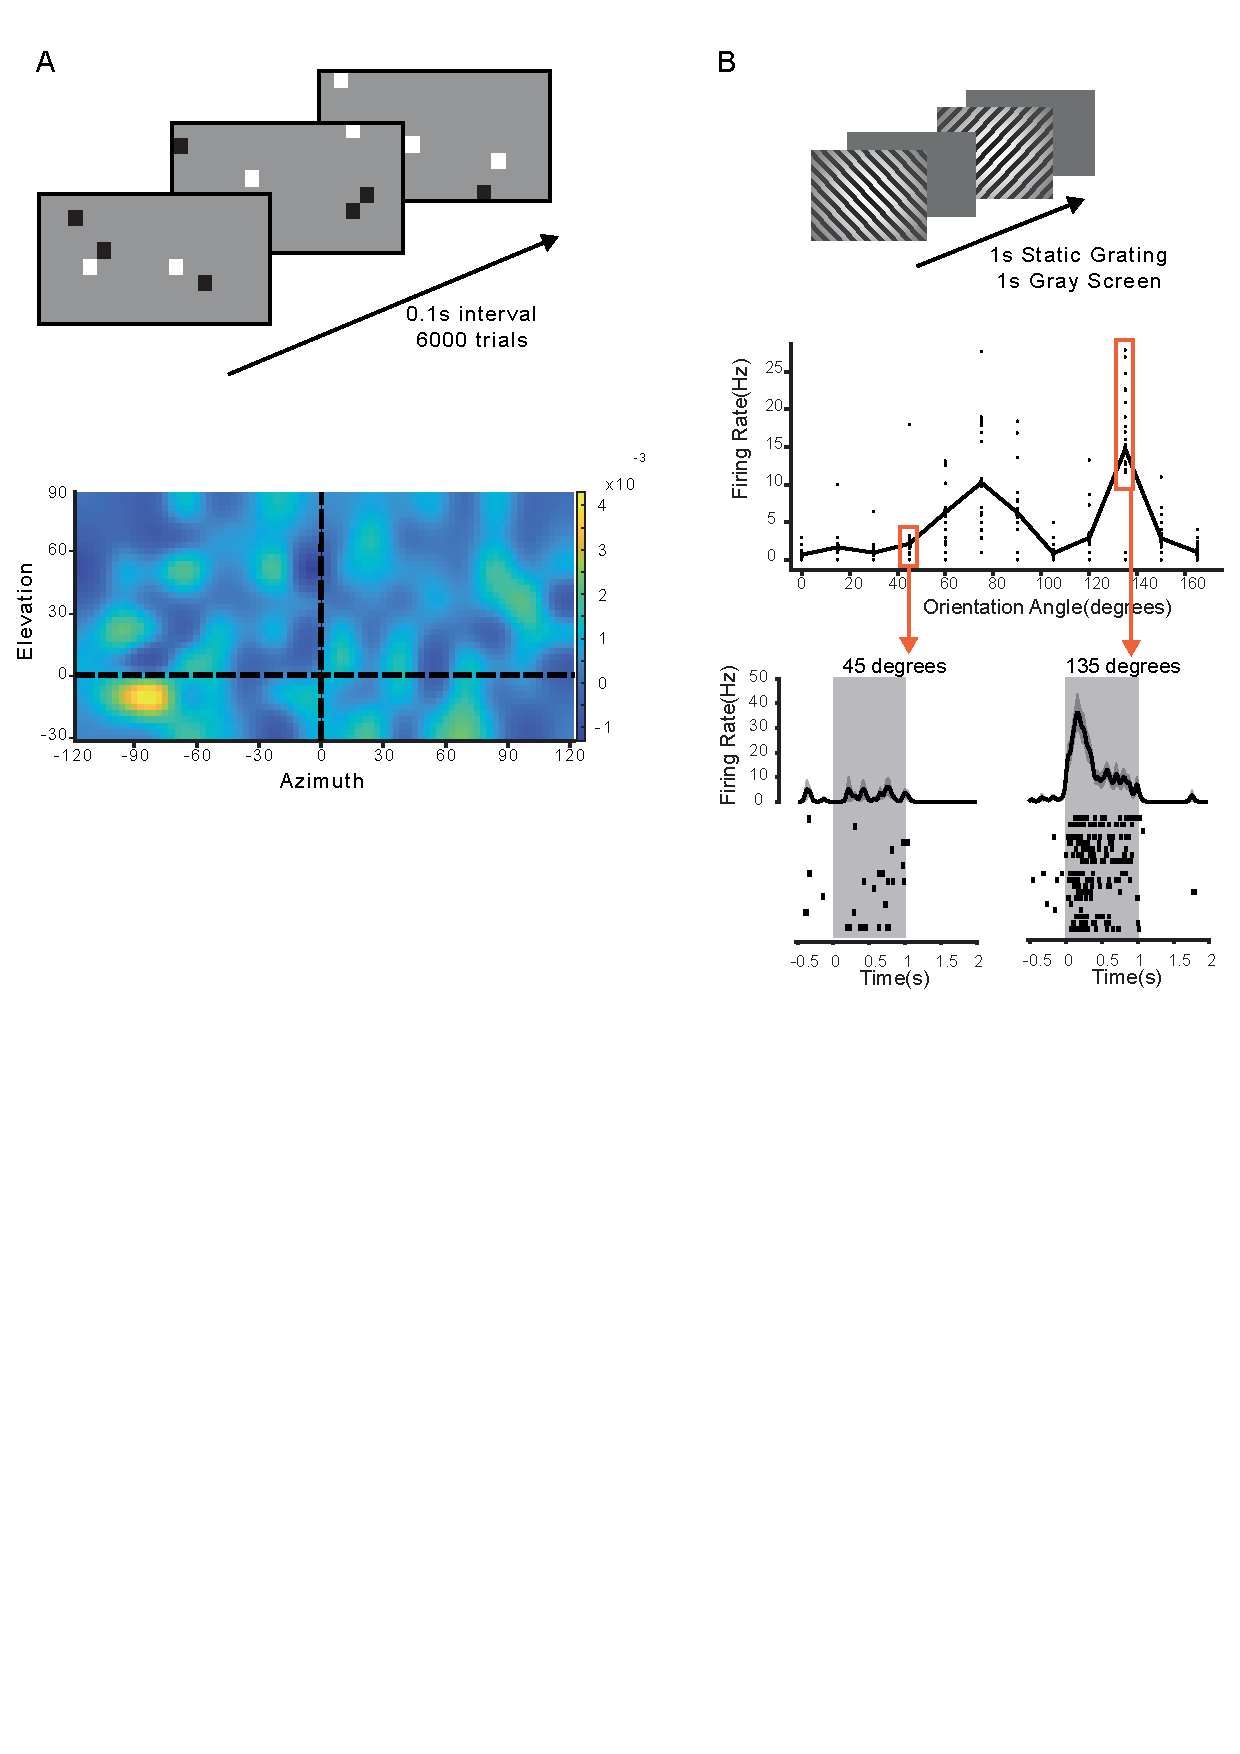
\includegraphics[width=1\linewidth]{figures//Chapter 2//Thesis Figures/fig4_RF_and_gratings.pdf}
    \caption{Visual Stimuli}
    \label{fig:placeholder}
\end{figure}

\subsection{Freely Moving in Open Field}
The experimented mouse is placed on top of an elevated round platform in 70 cm diameter for 30-50 minutes. The disk is surrounded by a 200 cm diameter circular wall with two patches of visual stimuli opposite to each other. Random rewards are dropped on the platform to encourage the mouse to explore the environment. An IR camera from above is used to track the animal's position and an IR LED is on the floor to synchronise between the videos and recordings.



\section{Preprocessing Pipeline}
\subsection{Recording Preprocessing}
The recording acquisition was done on spikeGLX on an acquisition PC. The LFP is extracted with catGT command line helper with a low-pass filter after phase shift correction. For spike sorting, spikeinterface is used to perform compression (zarr: wavPack compressor), pre-processing (standard phase shift correction, common reference averaging, remove bad channels with high noise), motion correction (spikeinterface's non-rigid method), spike sorting with kilosort 3 (acute recordings) and kilosort 4 (chronic recordings), and quality metrics (Fig 2.5 Ephys Preprocessing). Each day's recordings are all concatenated for spike sorting. In chronic recordings, unknown electric current issue caused the recordings to have error samples and made some recordings unusable. Such error is detected using sync channel and any recording samples after the error are removed before compression.

\subsection{Data Synchronisation}
The Neuropixel acuquisition PC records the electrophysiology data, and the behaviour PC displays stimuli and VR and records the behaviour variables and events (Fig 2.5 Behaviour and Stimulus). For synchronisation, an Arduino high frequency sync pulse is sent to Neuropixel acquisition PC and behaviour PC and a photodiode is placed in front of the screens where a stimulus quad is exhibited when stimuli are on). The data streams are aligned by the sync onset and offset to the Neuropixel clock. The real time of Bonsai visual stimuli and VR rendering are recorded by the photodiode and together with behaviour variables are aligned to Neuropixel clock. This method provides high redundancy of synchronisation which saved a few recordings having some information missing and allows correction for delays between bonsai and screen displays of stimuli (Fig 2.5). 

\subsection{Visual Response Analysis}
For checkboard stimulus, local field potential (LFP) signals in channels at different depths are extracted and power density is calculated first to give a rough guide of signature LFP signals in different regions. Current source density is calculated from LFP in response to checkboard (Fig 2.4C). In addition, power spectral density is calculated from the LFP in different frequency bands, 0.5-3Hz, 4-12Hz, 125-300Hz, 300-600Hz (Fig 2.4B).

 For sparse noise stimulus, the trial info is extracted as a matrix of azimuth x elevation x trial number. Peri-stimulus time histogram (PSTH) is first used to estimate responses of each unit at each trial. Single value decomposition is applied to the response matrix across trials with the stimulus matrix and separates the spatiotemporal responses of each unit and their stimulus weighting map across trials. The stimulus weighting map can be considered as the receptive field of a unit (Fig 2.3).

 For static grating stimulus, PSTH in firing rate with gaussian smoothing of each grating angle are plotted with raster plot -0.5s before the stimulus until 2s of stimulus on and preliminary tuning strengths are calculated from the absolute value of the difference between mean activities when stimulus is on and mean activities when stimulus is off (Fig 2.3).


\subsection{Spatial Tunning and Stability}
For the spatial tuning preliminary analysis, spikes are binned in 1 cm spanning 140cm each trial. Spike activities during running (>1 cm/s) are shuffled 1000 times circularly in the same lap and the unit is considered spatially-tuned if the difference between maximum and minimum values in the track is 95\% stronger than shuffled values. For stability measures, point-wise correlations are calculated between odd and even laps' averages, and first and second half's averages. For a stable cell, the stability correlations of real data are higher than 95\% of shuffled data. 

In some acute sessions, large shared difference between two parts of the same session is found amongst all neurons but the exact reason is not found and can be highly due to probe motion when the probes were not stable in early part of recordings. Therefore, a trunk of VR laps is removed to reduce its impact on the analysis.


\subsection{Register Probe to Brain Regions}
Both probes are inserted from visual cortex regions. Under this assumption, checkboard is a great tool (elicts large responses across visual cortex) to find the high power locations of 125-300Hz and 300-600Hz bands and the onset location of CSD analysis which should be the layer 4 and layer 5 of V1 and visual area P when a visual stimulus is presented. A second 125-300Hz and 300-600Hz bump in V1 probe is commonly CA1. In MEC probe, following visual area, a large bump in 4-12Hz (theta band) is commonly found. This analysis is further checked with the histology sections.
\begin{figure}
    \centering
    \includegraphics[width=1\linewidth]{figures//Chapter 2/fig3_probe_location_checkerboard.pdf}
    \caption{Register Brain Region to the Probe Based on Histology and Physiology}
    \label{fig:placeholder}
\end{figure}


\begin{figure}
    \centering
    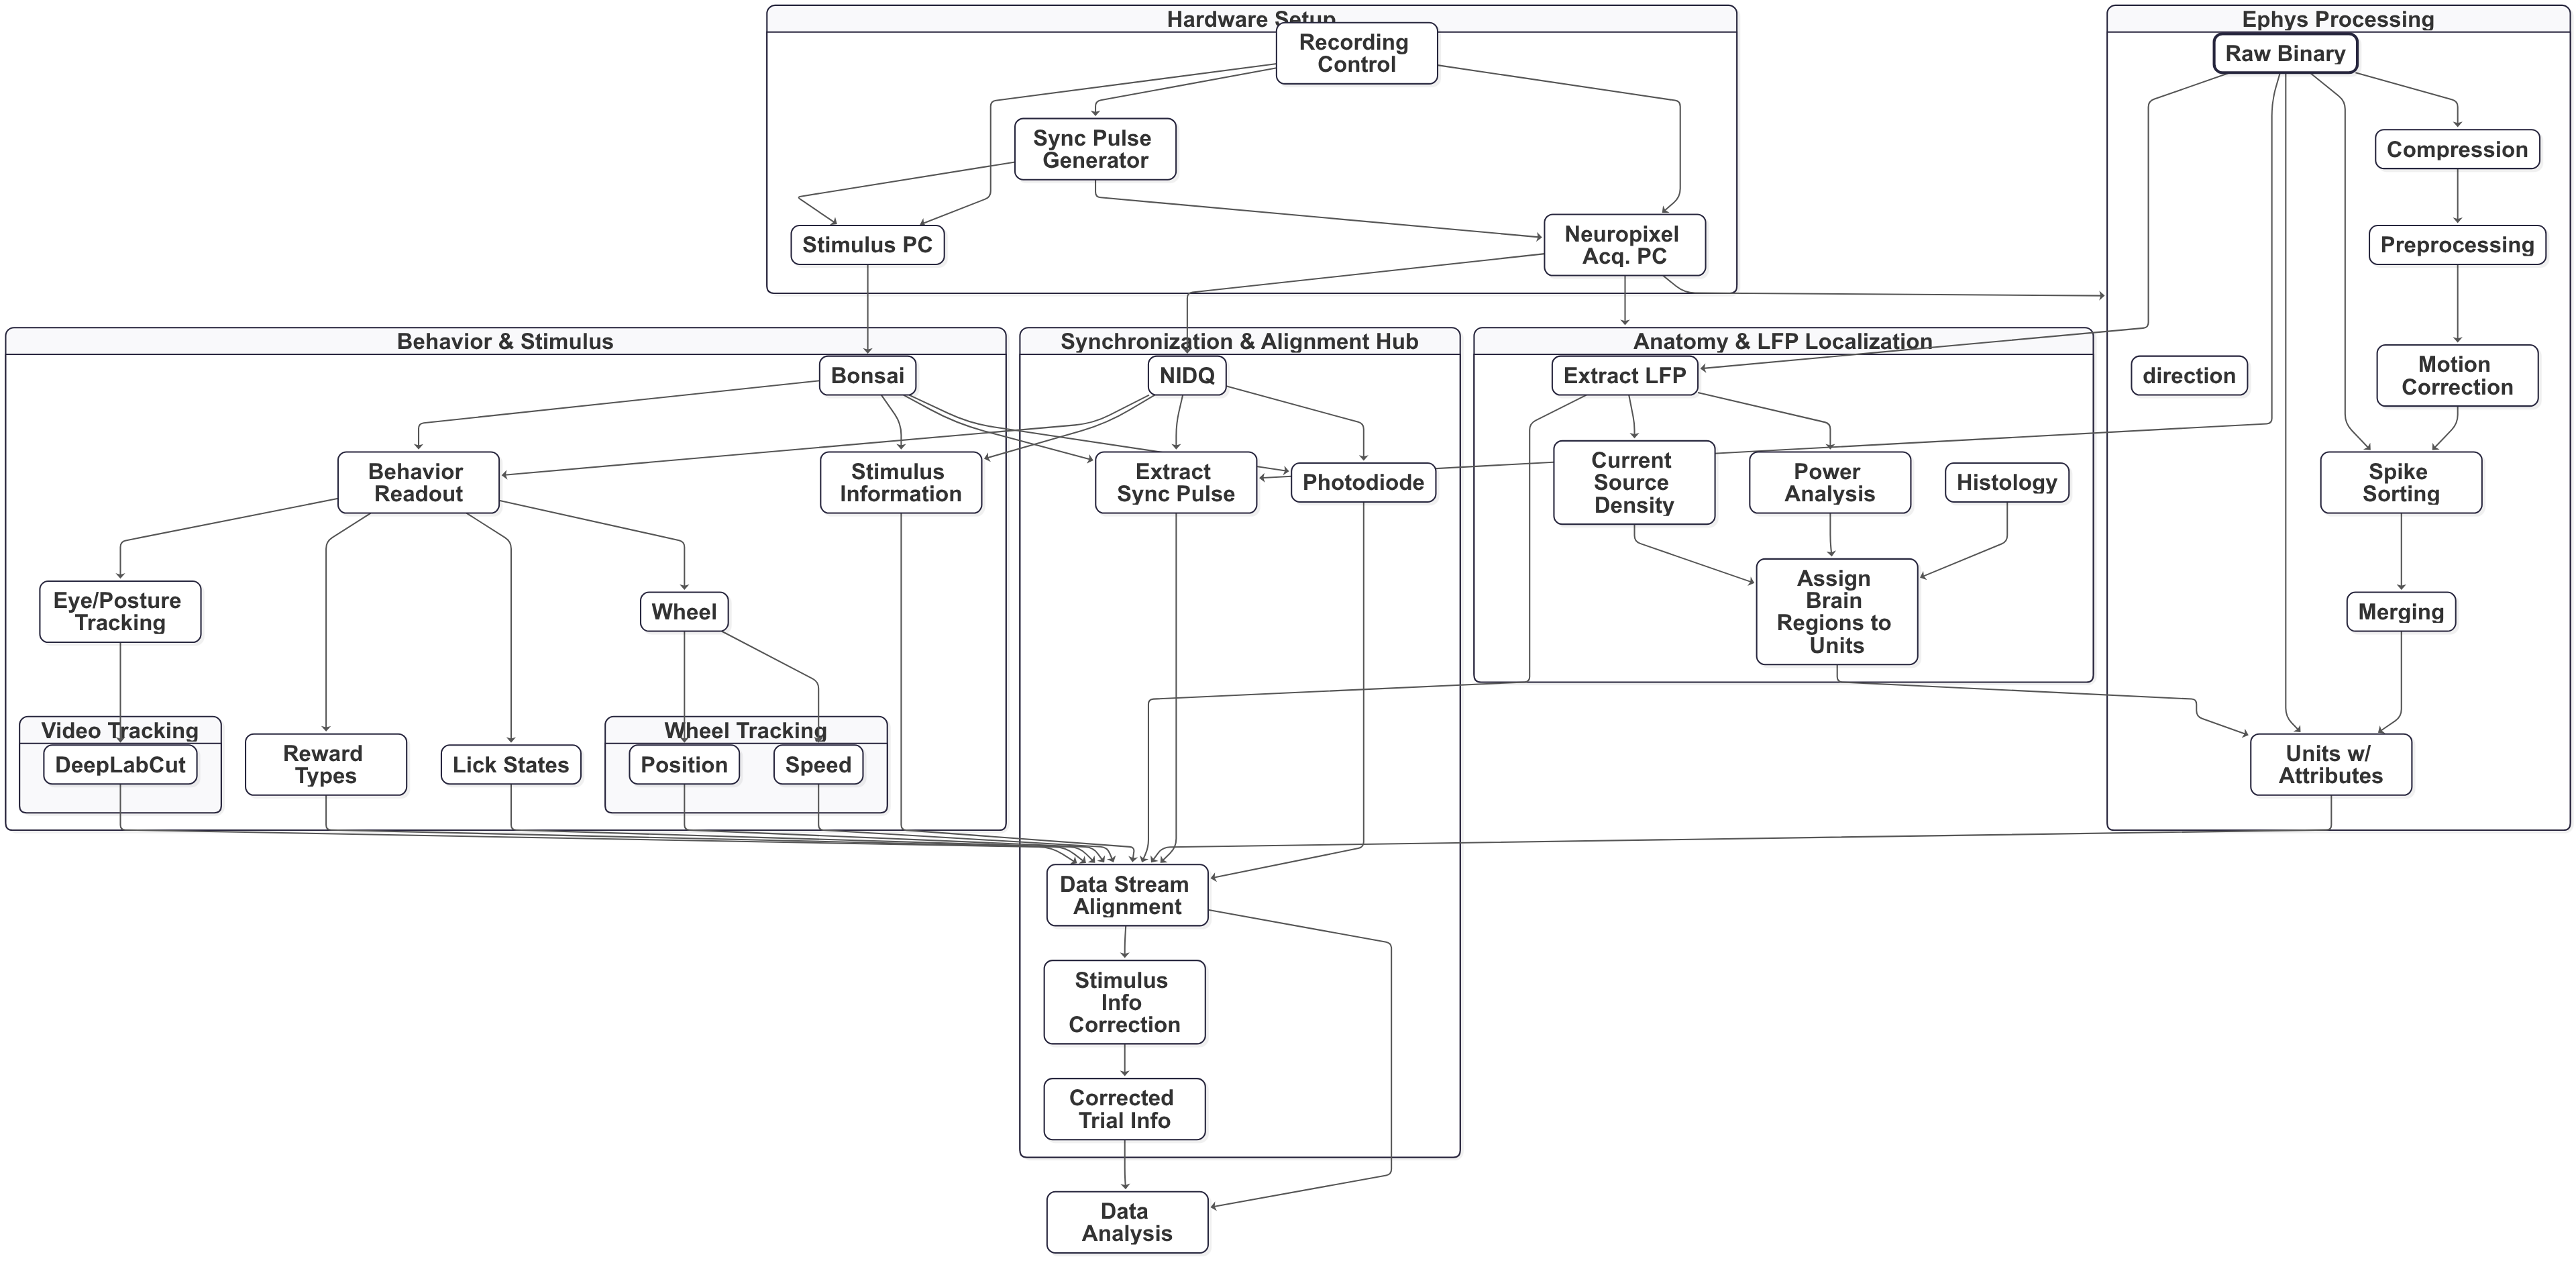
\includegraphics[width=1\linewidth]{figures//Chapter 2//plots/flow_chart_td.png}
    \caption{Experiment Data Preprocessing Pipeline}
    \label{fig:placeholder}
\end{figure}





\section{Histology}
Pilot mEC coordinates were first tested before behavioural training with head implanted on animals. A needle was dipped inside DiI and inserted into the mouse brain at ML –3.4 before the transverse sinus at a 10-degree angle from posterior to anterior with stereotax. The mouse was anaesthetized with 3.5\% isoflurane, and then euthanized by intraperitoneal injection of overdose pentobarbital. The mouse is perfused with saline and followed by 4\% paraformaldehyde (PFA). The brain was extracted and stored in 4\% PFA for one day after which it was washed with 1X PBS twice and placed in 30\% sucrose until it settled to the bottom of the bottle. The brain is frozen in OCT and cut into 50microns sagittal sections with a cryostat. The brain slices were mounted in DAPI solution and imaged with a fluorescence microscope. The slices were registered to the Allen Mouse Brain Atlas and the insertion tract was reconstructed by a MATLAB based software SHARP-Track (\href{https://github.com/cortex-lab/allenCCF}{https://github.com/cortex-lab/allenCCF}) (Fig 2.4D).

 In acute electrophysiology recording histology, the neuropixels were applied with same DiI or DiD or DiO before each recording session. The rest of the histology procedure is the same. Dyes at different fluorescent wavelengths can help distinguish corresponding sessions. For chronic recordings, only DiI is applied to all shanks.
